\section{Estratégias de Paralelização}
\label{sec:paralelizacao}

\subsection{Evolução da Estratégia de Paralelização}
\label{sec:discussao_inicial}

A abordagem inicial avaliada para explorar a dependência em \textit{wavefront} consistiu em avançar diagonalmente pela matriz utilizando apenas 2 \textit{threads}: uma encarregada de computar a linha horizontal e a outra a coluna vertical até a posição $(i, j)$ da diagonal (Figura~\ref{fig:estrategia_openmp}a). No entanto, essa estratégia revelou dois gargalos determinantes: a concorrência fica estritamente limitada a 2 \textit{threads} e o cálculo da coluna quebra a contiguidade de memória em C (\textit{row-major}), gerando um volume excessivo de \textit{cache misses}.

Para superar essas restrições, a solução adotada foi a \textbf{decomposição 2D em blocos} (\textit{tiling}) de tamanho fixo $\texttt{BLOCK\_SIZE} \times \texttt{BLOCK\_SIZE}$. Cada bloco é processado sequencialmente linha a linha por uma \textit{thread}, garantindo localidade espacial na cache L1d e permitindo que múltiplos blocos ao longo das anti-diagonais sejam escalonados simultaneamente entre muitos núcleos (Figura~\ref{fig:estrategia_openmp}b).

\subsection{Versão OpenMP: Decomposição em Blocos 2D}
\label{sec:openmp}

Para minimizar a sobrecarga de sincronização e manter alta localidade de referência, a matriz é dividida em blocos de $\texttt{BLOCK\_SIZE} \times \texttt{BLOCK\_SIZE}$ ($512 \times 512$). Internamente, cada bloco é processado sequencialmente linha a linha, favorecendo o \textit{hardware prefetcher} e residindo integralmente na cache da CPU.

O paralelismo ocorre entre blocos via tarefas dependentes (\texttt{\#pragma omp task depend(in: ...) depend(out: ...)}). A thread principal (\texttt{\#pragma omp single}) percorre a grade e despacha as tarefas ao escalonador do OpenMP, que gerencia dinamicamente o Grafo Acíclico Dirigido (DAG). Utiliza-se \textit{padding} na matriz de sincronização (\texttt{sync\_matrix}) para eliminar desvios condicionais nas bordas (Figura~\ref{fig:estrategia_openmp}c).

\begin{figure}[H]
\centering
\begin{minipage}[b]{0.31\textwidth}
\centering
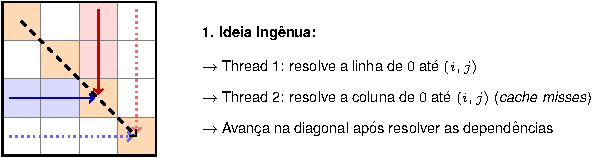
\includegraphics[width=\linewidth]{images/ideia_ingenua.pdf}
\caption*{(a) 2 \textit{threads} (ingênua).}
\end{minipage}\hfill
\begin{minipage}[b]{0.31\textwidth}
\centering
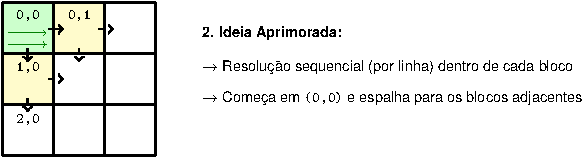
\includegraphics[width=\linewidth]{images/ideia_blocos.pdf}
\caption*{(b) Decomposição 2D.}
\end{minipage}\hfill
\begin{minipage}[b]{0.34\textwidth}
\centering
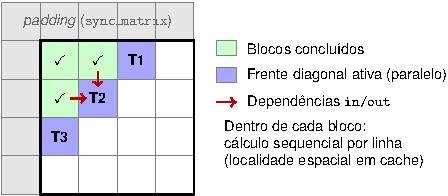
\includegraphics[width=\linewidth]{images/omp_wavefront.pdf}
\caption*{(c) Avanço diagonal com \textit{padding}.}
\end{minipage}
\caption{Evolução da paralelização em memória compartilhada (OpenMP): (a) restrição a 2 \textit{threads}; (b) blocos 2D escaláveis; (c) avanço diagonal com tarefas dependentes e \textit{padding}.}
\label{fig:estrategia_openmp}
\end{figure}
